%12_dijkstra.tex
%notes for the course COMS10007 taught at the University of Bristol
%Conor Houghton conor.houghton@bristol.ac.uk

%To the extent possible under law, the author has dedicated all copyright 
%and related and neighboring rights to these notes to the public domain 
%worldwide. These notes are distributed without any warranty. 

\documentclass[11pt,a4paper]{scrartcl}
\typearea{12}
\usepackage{graphicx}
\usepackage{listings}
\usepackage{tikz}
%\usepackage{tikz-qtree}                                                        
\usetikzlibrary{positioning}
\lstset{language=C}
\usepackage{fancyhdr}
\pagestyle{fancy}
\lfoot{\texttt{github.com/conorhoughton/COMS10007}}
\lhead{COMS10007 - algorithms 11\_dijkstra (n) - Conor}
\begin{document}

\subsection*{12- graphs two\footnote{\texttt{http://github.com/conorhoughton/COMS10001}} - DRAFT}

In these notes we will learn about two constructive algorithms; the
first, Fleury's Algorithm, allows an Eulerian path to be constructed
if one exists and the second, Dijkstra's Algorithm, a very famous and
useful algorithm, allows us to find the shortest path through a
weighted graph. We won't look at a formal proof in either case, but
for both the algorithms are compelling enough that it is reasonably
clear how a proof might work.

\subsubsection*{Fleury's algorithm}


\begin{figure}
\begin{center}
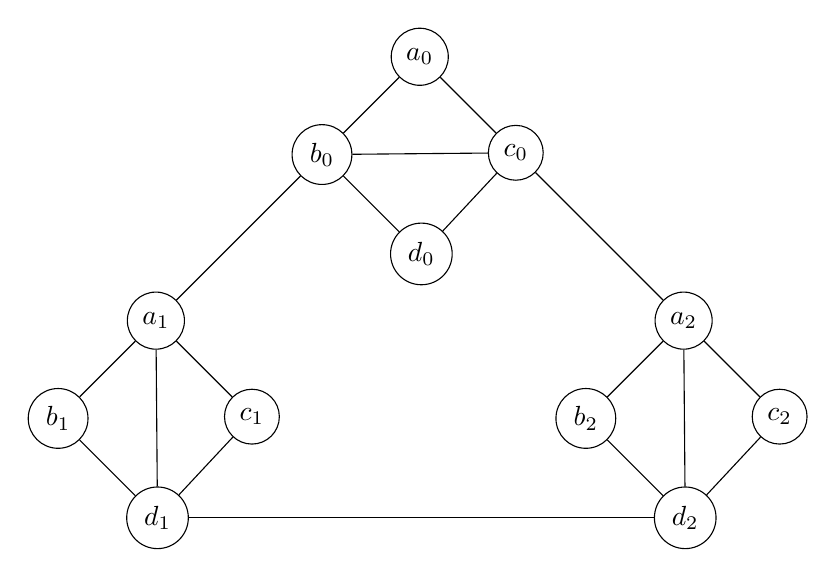
\begin{tikzpicture}
\node[draw,circle](a){$a_0$};
\node[draw,circle, below left= 1cm of a](b){$b_0$};
\node[draw,circle, below right =1cm of a](c){$c_0$};
\node[draw,circle, below right = 1cm of b](d){$d_0$};
\path (a) edge (b);
\path (a) edge (c);
\path (b) edge (d);
\path (c) edge (d);
\path (b) edge (c);

\node[draw,circle,below left=4cm of a](a1){$a_1$};
\node[draw,circle, below left= 1cm of a1](b1){$b_1$};
\node[draw,circle, below right =1cm of a1](c1){$c_1$};
\node[draw,circle, below right = 1cm of b1](d1){$d_1$};
\path (a1) edge (b1);
\path (a1) edge (c1);
\path (b1) edge (d1);
\path (c1) edge (d1);
\path (a1) edge (d1);


\node[draw,circle,below right=4cm of a](a2){$a_2$};
\node[draw,circle, below left= 1cm of a2](b2){$b_2$};
\node[draw,circle, below right =1cm of a2](c2){$c_2$};
\node[draw,circle, below right = 1cm of b2](d2){$d_2$};
\path (a2) edge (b2);
\path (a2) edge (c2);
\path (b2) edge (d2);
\path (c2) edge (d2);
\path (a2) edge (d2);

\path (d1) edge (d2);
\path (b) edge (a1);
\path (c) edge (a2);



\end{tikzpicture}
\end{center}
\caption{A graph that usefully illustrates Fleury's algorithm. \label{fig:graph}}
\end{figure}




Imagine trying to find an Eulerian cycle for the graph in
Fig.~\ref{fig:graph}, but without thinking about it too hard; say you
start at $a_0$ and go to $b_0$ before heading off for $a_1$, then
$b_1$ and $d_1$ before going hog-wild and going on to $d_2$, the
situation you find yourself in is illustrated in
Fig.~\ref{fig:graph_hw}; it is clear the situation is hopeless, there
is no way to return to the subscript-1 group of nodes to traverse the
edges between $a_1$ and $d_1$, $a_1$ and $c_1$ and $d_1$ and
$c_1$. These should have been finished up before leaving for the
subscript-2 nodes. The sequence $a_0b_0a_1d_1a_1c_1d_1d_2$, but even
if the subscript-2 nodes are all carefully visited,
$d_2b_2a_2c_2d_2a_2$ before returning to the subscript-0 nodes,
$a_2c_0$ it is still possible to mess up by returning to $a_0$ before
visiting the edges $c_0d_0b_0c_0$.

Playing with this example shows that the problem is with creating
\lq{}islands\rq{}, a node, or group of nodes, you can't return to
because all the links to them have been used up. At this point it is
useful to define a \textsl{connected} graph and a \textsl{bridge}. A
graph is connected if, for every pair of nodes $a$ and $b$ there is a
trail from $a$ to $b$. Now, a bridge is an edge which, if it was
removed, would leave the graph disconnected; examples are given in
Fig.~\ref{fig:bridges}. Now imagine removing the edges as you traverse
them, if you remove a bridge then you cannot return to the nodes left
behind, so when trying to walk an Eulerian path it is important not to
remove bridges if there are still edges to walk. This is basically
Fleury's algorithm, it says that you should never choose a bridge if
there is a choice, this is summarized in Table~\ref{table:fleury}.

\begin{table}
\begin{itemize}
\item If a node has an edge that isn't a bridge take that.
\item As you traverse each edge remove it.
\item If you remove the last edge at a node, remove the node.
\end{itemize}
\caption{Fleury's algorithm \label{table:fleury}}
\end{table}
  
\begin{figure}
\begin{center}
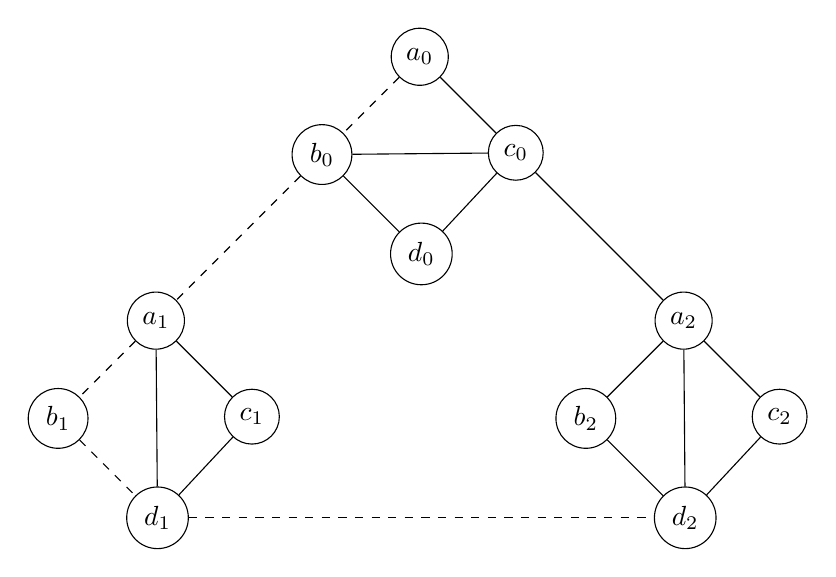
\begin{tikzpicture}
\node[draw,circle](a){$a_0$};
\node[draw,circle, below left= 1cm of a](b){$b_0$};
\node[draw,circle, below right =1cm of a](c){$c_0$};
\node[draw,circle, below right = 1cm of b](d){$d_0$};
\path (a) edge[dashed] (b);
\path (a) edge (c);
\path (b) edge (d);
\path (c) edge (d);
\path (b) edge (c);

\node[draw,circle,below left=4cm of a](a1){$a_1$};
\node[draw,circle, below left= 1cm of a1](b1){$b_1$};
\node[draw,circle, below right =1cm of a1](c1){$c_1$};
\node[draw,circle, below right = 1cm of b1](d1){$d_1$};
\path (a1) edge[dashed] (b1);
\path (a1) edge (c1);
\path (b1) edge[dashed] (d1);
\path (c1) edge (d1);
\path (a1) edge (d1);


\node[draw,circle,below right=4cm of a](a2){$a_2$};
\node[draw,circle, below left= 1cm of a2](b2){$b_2$};
\node[draw,circle, below right =1cm of a2](c2){$c_2$};
\node[draw,circle, below right = 1cm of b2](d2){$d_2$};
\path (a2) edge (b2);
\path (a2) edge (c2);
\path (b2) edge (d2);
\path (c2) edge (d2);
\path (a2) edge (d2);

\path (d1) edge[dashed] (d2);
\path (b) edge[dashed] (a1);
\path (c) edge (a2);



\end{tikzpicture}
\end{center}
\caption{A bad start to finding an Eulerian path, the edges already traversed are dashed.\label{fig:graph_hw}}
\end{figure}





\begin{figure}
\begin{center}
\begin{tikzpicture}
\node[draw,circle](a){};
\node[draw,circle, below left= 1cm of a](b){};
\node[draw,circle, below right =1cm of a](c){};
\node[draw,circle, below right = 1cm of b](d){};
\path (a) edge (b);
\path (a) edge (c);
\path (b) edge (d);
\path (c) edge (d);
\path (b) edge (c);

\node[draw,circle,right=4cm of a](a1){};
\node[draw,circle, below left= 1cm of a1](b1){};
\node[draw,circle, below right =1cm of a1](c1){};
\node[draw,circle, below right = 1cm of b1](d1){};
\path (a1) edge (b1);
\path (a1) edge (c1);
\path (b1) edge (d1);
\path (c1) edge (d1);
\path (a1) edge (d1);


\node[draw,circle,right=4cm of a1](a2){};

\path (a1) edge[dashed] (a2);
\path (c) edge[dashed] (b1);

\end{tikzpicture}
\end{center}
\caption{The two dashed edges are bridges since deleting either of them would make the graph disconnected. \label{fig:bridges}}
\end{figure}

\subsubsection*{Dijkstra's algorithm}

The problem Dijkstra's algorithm solves is how to find the shortest
path through a weighted graph. Consider the graph in
Fig.~\ref{fig:weighted}; Dijksktra's algorithm solves, for example, the
problem of how to go from ($a$) to ($e$) by the shortest route. The
actual shortest route is given in Fig.~\ref{fig:shortest}.

\begin{figure}
\begin{center}
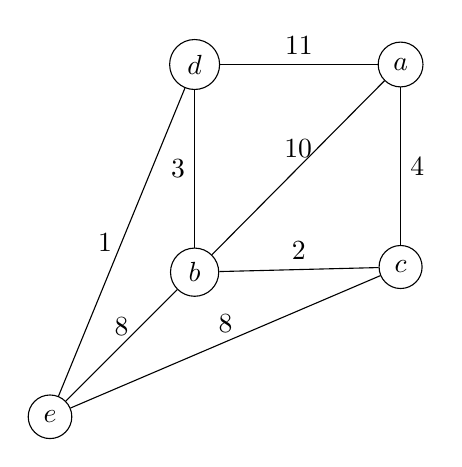
\begin{tikzpicture}
\node[draw,circle](a){$a$};
\node[draw,circle, below      =2cm of a](c){$c$};
\node[draw,circle, left = 2cm of a](d){$d$};
\node[draw,circle, below = 2 cm of d](b){$b$};
\node[draw,circle, below left = 2 cm of b](e){$e$};
\path (a) edge node[above]{10} (b);
\path (a) edge node[right]{4} (c);
\path (b) edge node[left]{3} (d);
\path (a) edge node[above]{11} (d);
\path (b) edge node[above]{2} (c);
\path (b) edge node[above]{8} (e);
\path (d) edge node[left]{1} (e);
\path (c) edge node[above]{8} (e);
\end{tikzpicture}
\end{center}
\caption{A weighted graph \label{fig:weighted}}
\end{figure}


\begin{figure}
\begin{center}
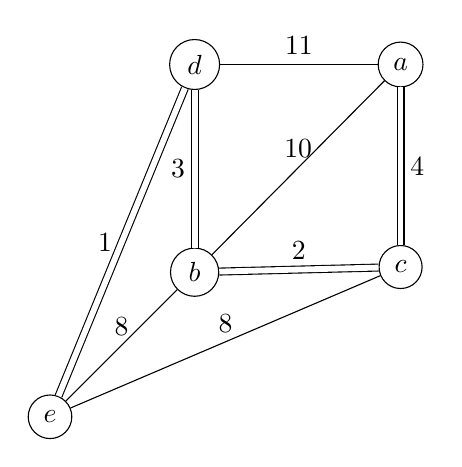
\begin{tikzpicture}
\node[draw,circle](a){$a$};
\node[draw,circle, below      =2cm of a](c){$c$};
\node[draw,circle, left = 2cm of a](d){$d$};
\node[draw,circle, below = 2 cm of d](b){$b$};
\node[draw,circle, below left = 2 cm of b](e){$e$};
\path (a) edge node[above]{10} (b);
\draw[double, double distance between line centers=0.25em] (a) -- node[right]{4} (c);
\path (b) edge[double, double distance between line centers=0.25em] node[left]{3} (d);
\path (a) edge node[above]{11} (d);
\path (b) edge[double, double distance between line centers=0.25em] node[above]{2} (c);
\path (b) edge node[above]{8} (e);
\path (d) edge[double, double distance between line centers=0.25em] node[left]{1} (e);
\path (c) edge node[above]{8} (e);
\end{tikzpicture}
\end{center}
\caption{Shortest path: the double lines mark the shortest path \label{fig:shortest}}
\end{figure}

Now if you start at ($a$) you can work out directly the distance using
one edge to all the nodes adjacent to $a$, this is given in
Fig.~\ref{fig:near_a}. Let's attribute a distance of $D(x)$ to a node
$x$ and call the length of the edge between nodes $x$ and $y$
$D(x,y)$. Thus, after looking at the nodes adjacent to $a$, we have
$D(b)=10$, that is the distance ten is attributed to ($b$). This is
not the actual shortest distance from $a$ to $b$, there is a shorter
path that goes by way of $c$ which would give a distance of six. Thus,
the next step is to select another node, let's call it $x$ and
update the distances to its neighbours, so, for example, if $y$ is a neighbour of $x$ and $D(x)+D(x,y)<D(y)$ then $D(y)$ should be updated to this new, shorted, distance, $D(y)\rightarrow D(x)+D(x,y)$.

Now, this process might reduce some distances, but will never reduce
the distance to the node with the lowest $D(x)$; thus, if we choose
$x$ to be this lowest distance node, after we update all its connected
nodes, we can cross it off and not look at it again. In the case of
the graph we have been looking at, the lowest node in
Fig.~\ref{fig:near_a} is $c$, so the next step is to look at its
neighbours, $a$ has already been crossed off, so $D(b)$ is updated to
six and $D(e)$ to 12. This situation is shown in
Fig.~\ref{fig:after_c}. At this point $b$ has the smallest assigned
distance, so it is considered next, since $D(b)+D(b,e)=14>12$, $D(e)$
isn't changed, but $D(d)$ is set to nine. This is shown in
Fig.~\ref{fig:final_moves}\textbf{A}. Now the smallest node is $d$, updating
its neighbours reduces the distance to $e$ to 10, see
Fig.~\ref{fig:final_moves}\textbf{B}. Since $e$ is now the unchecked node
with the smallest distance we are done.

\begin{figure}
\begin{center}
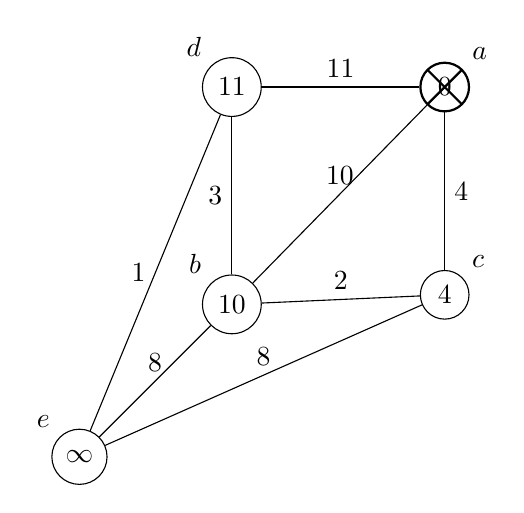
\begin{tikzpicture}
[cross/.style={path picture={ \draw[black] (path picture bounding
      box.south east) -- (path picture bounding box.north west) (path
      picture bounding box.south west) -- (path picture bounding
      box.north east); }}] \node[draw,thick,circle,cross,label=above
  right:$a$](a){$0$}; \node[draw,circle, below =2cm of a,label=above
  right:$c$](c){$4$}; \node[draw,circle, left = 2cm of a,label=above
  left:$d$](d){$11$}; \node[draw,circle, below = 2 cm of d,label=above
  left:$b$](b){$10$}; \node[draw,circle, below left = 2 cm of
  b,label=above left:$e$](e){$\infty$}; \path (a) edge node[above]{10}
(b); \path (a) edge node[right]{4} (c); \path (b) edge node[left]{3}
(d); \path (a) edge node[above]{11} (d); \path (b) edge node[above]{2}
(c); \path (b) edge node[above]{8} (e); \path (d) edge node[left]{1}
(e); \path (c) edge node[above]{8} (e);
\end{tikzpicture}
\end{center}
\caption{This shows the distance to the nodes adjacent to ($a$)
  directly along one edge, the node labels have been moved outside the
  nodes so that the distances can be written inside. The distance to
  ($e$) has been marked as $\infty$ because we haven't found a route
  to ($e$) yet. $(a)$ has a cross in it since we have already looked
  at its nearest neighbours. \label{fig:near_a}}
\end{figure}

\begin{figure}
\begin{center}
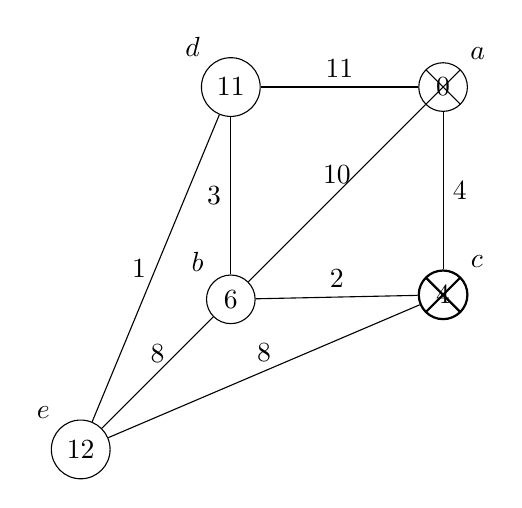
\begin{tikzpicture}
[cross/.style={path picture={ \draw[black] (path picture bounding
      box.south east) -- (path picture bounding box.north west) (path
      picture bounding box.south west) -- (path picture bounding
      box.north east); }}] 
\node[draw,circle,cross,label=above  right:$a$](a){$0$}; 
\node[draw,thick,cross,circle, below =2cm of a,label=above  right:$c$](c){$4$}; 
\node[draw,circle, left = 2cm of a,label=above  left:$d$](d){$11$}; 
\node[draw,circle, below = 2 cm of d,label=above left:$b$](b){$6$}; 
\node[draw,circle, below left = 2 cm of b,label=above left:$e$](e){$12$}; 
\path (a) edge node[above]{10}
(b); \path (a) edge node[right]{4} (c); \path (b) edge node[left]{3}
(d); \path (a) edge node[above]{11} (d); \path (b) edge node[above]{2}
(c); \path (b) edge node[above]{8} (e); \path (d) edge node[left]{1}
(e); \path (c) edge node[above]{8} (e);
\end{tikzpicture}
\end{center}
\caption{This shows the situation after $c$'s neighbours have been considered. \label{fig:after_c}}
\end{figure}


\begin{figure}
\begin{center}
$\begin{array}{lclc}
\textbf{A}&&\textbf{B}&\\
&
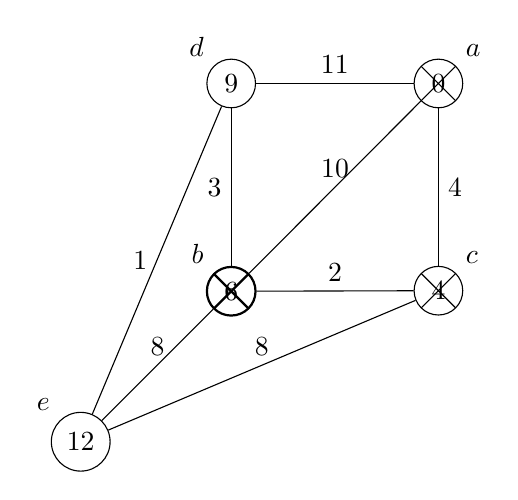
\begin{tikzpicture}
[cross/.style={path picture={ \draw[black] (path picture bounding
      box.south east) -- (path picture bounding box.north west) (path
      picture bounding box.south west) -- (path picture bounding
      box.north east); }}] 
\node[draw,circle,cross,label=above  right:$a$](a){$0$}; 
\node[draw,cross,circle, below =2cm of a,label=above  right:$c$](c){$4$}; 
\node[draw,circle, left = 2cm of a,label=above  left:$d$](d){$9$}; 
\node[draw,thick,cross,circle, below = 2 cm of d,label=above left:$b$](b){$6$}; 
\node[draw,circle, below left = 2 cm of b,label=above left:$e$](e){$12$}; 
\path (a) edge node[above]{10}
(b); \path (a) edge node[right]{4} (c); \path (b) edge node[left]{3}
(d); \path (a) edge node[above]{11} (d); \path (b) edge node[above]{2}
(c); \path (b) edge node[above]{8} (e); \path (d) edge node[left]{1}
(e); \path (c) edge node[above]{8} (e);
\end{tikzpicture}
&&
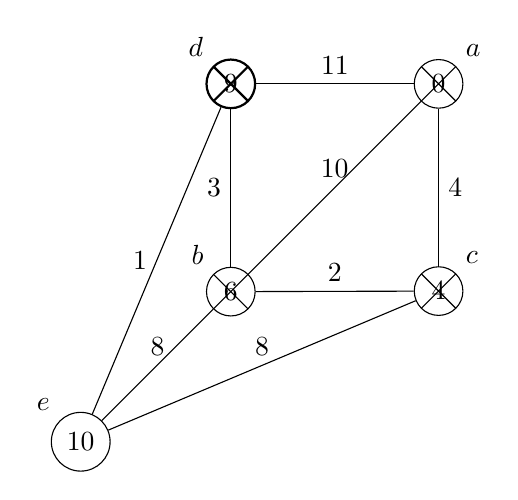
\begin{tikzpicture}
[cross/.style={path picture={ \draw[black] (path picture bounding
      box.south east) -- (path picture bounding box.north west) (path
      picture bounding box.south west) -- (path picture bounding
      box.north east); }}] 
\node[draw,circle,cross,label=above  right:$a$](a){$0$}; 
\node[draw,cross,circle, below =2cm of a,label=above  right:$c$](c){$4$}; 
\node[draw,circle,thick,cross, left = 2cm of a,label=above  left:$d$](d){$9$}; 
\node[draw,circle, cross,below = 2 cm of d,label=above left:$b$](b){$6$}; 
\node[draw,circle, below left = 2 cm of b,label=above left:$e$](e){$10$}; 
\path (a) edge node[above]{10}
(b); \path (a) edge node[right]{4} (c); \path (b) edge node[left]{3}
(d); \path (a) edge node[above]{11} (d); \path (b) edge node[above]{2}
(c); \path (b) edge node[above]{8} (e); \path (d) edge node[left]{1}
(e); \path (c) edge node[above]{8} (e);
\end{tikzpicture}
\end{array}$
\end{center}
\caption{This shows the situation after (\textbf{A}) $b$'s and
  (\textbf{B}) $d$'s neighbours have been considered. At this point
  $e$, the target node, is the available node with the lowest assigned
  distance, so the algorithm is done and the shortest path is
  ten. \label{fig:final_moves}}
\end{figure}

It would have been easy to keep track during the algorithm of the node
preceding a given node in the shortest path; this would allow the path to be retraced afterwards. This is shown in Fig.~\ref{fig:path}. A function to implement Dijkstra's algorithm and store the path, can be seen at Table~\ref{c_dijkstra}.


\begin{figure}
\begin{center}

$\begin{array}{lclc}
\textbf{A}&&\textbf{B}&\\
&
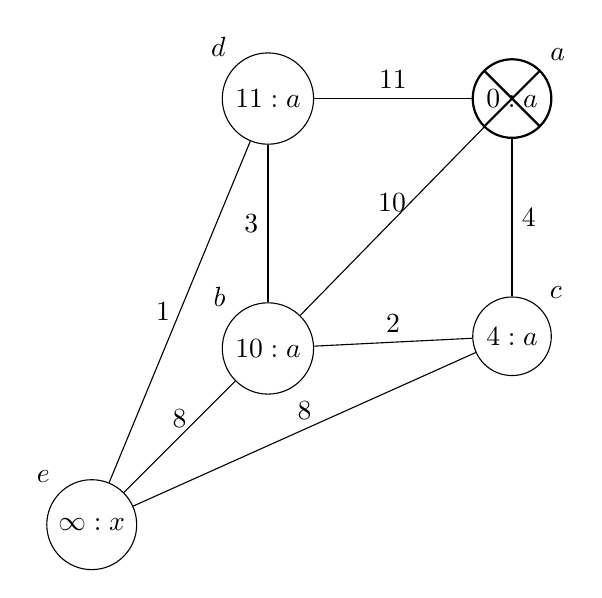
\begin{tikzpicture}
[cross/.style={path picture={ \draw[black] (path picture bounding
      box.south east) -- (path picture bounding box.north west) (path
      picture bounding box.south west) -- (path picture bounding
      box.north east); }}] \node[draw,thick,circle,cross,label=above
  right:$a$](a){$0:a$}; \node[draw,circle, below =2cm of a,label=above
  right:$c$](c){$4:a$}; \node[draw,circle, left = 2cm of a,label=above
  left:$d$](d){$11:a$}; \node[draw,circle, below = 2 cm of d,label=above
  left:$b$](b){$10:a$}; \node[draw,circle, below left = 2 cm of
  b,label=above left:$e$](e){$\infty:x$}; \path (a) edge node[above]{10}
(b); \path (a) edge node[right]{4} (c); \path (b) edge node[left]{3}
(d); \path (a) edge node[above]{11} (d); \path (b) edge node[above]{2}
(c); \path (b) edge node[above]{8} (e); \path (d) edge node[left]{1}
(e); \path (c) edge node[above]{8} (e);
\end{tikzpicture}
&&
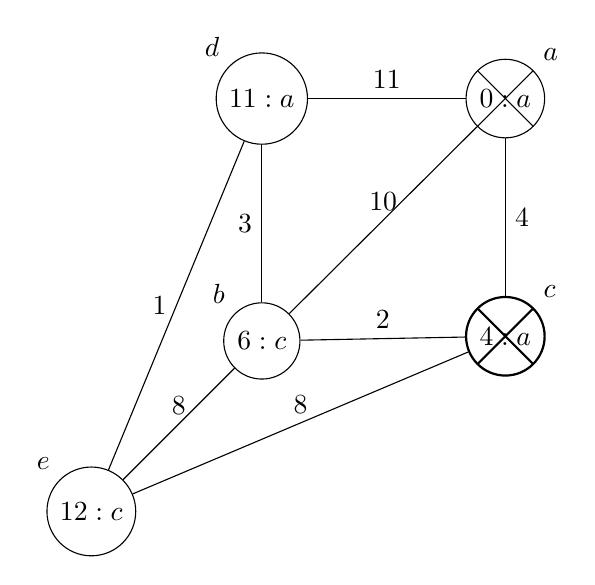
\begin{tikzpicture}
[cross/.style={path picture={ \draw[black] (path picture bounding
      box.south east) -- (path picture bounding box.north west) (path
      picture bounding box.south west) -- (path picture bounding
      box.north east); }}] 
\node[draw,circle,cross,label=above  right:$a$](a){$0:a$}; 
\node[draw,thick,cross,circle, below =2cm of a,label=above  right:$c$](c){$4:a$}; 
\node[draw,circle, left = 2cm of a,label=above  left:$d$](d){$11:a$}; 
\node[draw,circle, below = 2 cm of d,label=above left:$b$](b){$6:c$}; 
\node[draw,circle, below left = 2 cm of b,label=above left:$e$](e){$12:c$}; 
\path (a) edge node[above]{10}
(b); \path (a) edge node[right]{4} (c); \path (b) edge node[left]{3}
(d); \path (a) edge node[above]{11} (d); \path (b) edge node[above]{2}
(c); \path (b) edge node[above]{8} (e); \path (d) edge node[left]{1}
(e); \path (c) edge node[above]{8} (e);
\end{tikzpicture}\\
\textbf{C}&&\textbf{D}&\\
&
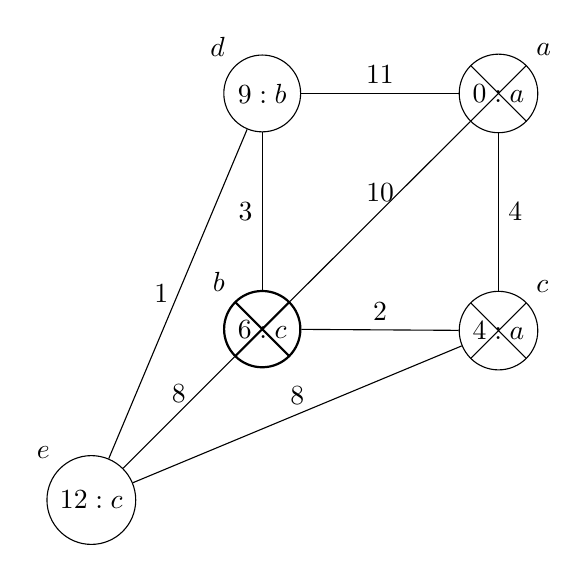
\begin{tikzpicture}
[cross/.style={path picture={ \draw[black] (path picture bounding
      box.south east) -- (path picture bounding box.north west) (path
      picture bounding box.south west) -- (path picture bounding
      box.north east); }}] 
\node[draw,circle,cross,label=above  right:$a$](a){$0:a$}; 
\node[draw,cross,circle, below =2cm of a,label=above  right:$c$](c){$4:a$}; 
\node[draw,circle, left = 2cm of a,label=above  left:$d$](d){$9:b$}; 
\node[draw,thick,cross,circle, below = 2 cm of d,label=above left:$b$](b){$6:c$}; 
\node[draw,circle, below left = 2 cm of b,label=above left:$e$](e){$12:c$}; 
\path (a) edge node[above]{10}
(b); \path (a) edge node[right]{4} (c); \path (b) edge node[left]{3}
(d); \path (a) edge node[above]{11} (d); \path (b) edge node[above]{2}
(c); \path (b) edge node[above]{8} (e); \path (d) edge node[left]{1}
(e); \path (c) edge node[above]{8} (e);
\end{tikzpicture}
&&
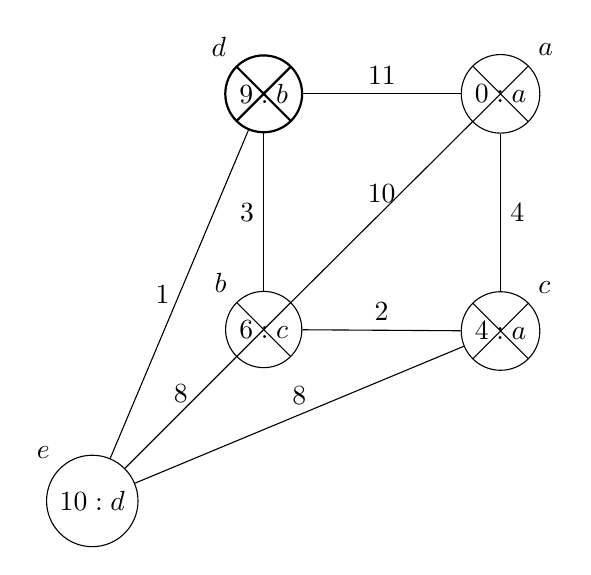
\begin{tikzpicture}
[cross/.style={path picture={ \draw[black] (path picture bounding
      box.south east) -- (path picture bounding box.north west) (path
      picture bounding box.south west) -- (path picture bounding
      box.north east); }}] 
\node[draw,circle,cross,label=above  right:$a$](a){$0:a$}; 
\node[draw,cross,circle, below =2cm of a,label=above  right:$c$](c){$4:a$}; 
\node[draw,circle,thick,cross, left = 2cm of a,label=above  left:$d$](d){$9:b$}; 
\node[draw,circle, cross,below = 2 cm of d,label=above left:$b$](b){$6:c$}; 
\node[draw,circle, below left = 2 cm of b,label=above left:$e$](e){$10:d$}; 
\path (a) edge node[above]{10}
(b); \path (a) edge node[right]{4} (c); \path (b) edge node[left]{3}
(d); \path (a) edge node[above]{11} (d); \path (b) edge node[above]{2}
(c); \path (b) edge node[above]{8} (e); \path (d) edge node[left]{1}
(e); \path (c) edge node[above]{8} (e);
\end{tikzpicture}
\end{array}$
\end{center}
\caption{Here along with the assigned distance the previous node is
  tracked, if the assigned distance is updated, so is the previous
  node; $x$ is used if there is no previous node, and $a$ is given $a$ as the previous node because it is the start of the path. Running backwards along the nodes we see the shortest path is $edbca$. \label{fig:path}}
\end{figure}


\begin{table}
\begin{lstlisting}[numbers=left]
int dijkstra(int a[n][n],int route[n])
{  
  int i, available[n], distances[n],current=0,next,min_distance;

  for(i=0;i<n;i++) {
    route[n]=0;
    available[i]=1;
    distances[i]=inf;
  }
  
  distances[0]=0;

  while(current!=n-1){
    available[current]=0;

    for(i=1;i<n;i++){
      if(available[i]&& distances[i]>distances[current]+a[i][current]){
	distances[i]=distances[current]+a[i][current];
	route[i]=current;
      }
    }
      
    next=current;
    min_distance=inf;
    for(i=1;i<n;i++){
      if(available[i]&&distances[i]<min_distance){
	next=i;
	min_distance=distances[i];
      }
    }
    current=next;
  }
  return distances[n-1];
} 
\end{lstlisting}
\caption{This works out the minimum distance from the 0th node to the \texttt{n-1}th node using the distance matrix \texttt{a}; it assumes \texttt{n}, the number of nodes, is a global variable. This function can been seen in action in \texttt{
    dijkstra.c}. \label{c_dijkstra}}
\end{table}

It is interesting that Dijkstra's algorithm does not use the identity
of the target node. Starting with the starting node it spreads
knowledge of the shortest path outwards through the graph and
terminates when the target node is the available node with the
shortest assigned distance.

\end{document}
